\chapter{Experiments}
\label{chap:exp}
In this chapter, we will show some experiment results to proof the effectiveness of our method. Section \ref{sec:onsetnormexp} deals with the onset deviation problem highlighted in Section \ref{sec:normalize}. Section \ref{sec:paramselect} discusses how various parameters in our system are chosen. Section \ref{sec:turing} describes a subjective test to test if audience can or can't identify the difference between generated and human performances.


\section{Onset Deviation Normalization}
\label{sec:onsetnormexp}
%\framebox{TODO:onset deviation problem review}
As mentioned in Section \ref{sec:normalize}, a bad normalization method will usually result in unreasonable high onset deviation. To overcome this challenge, we proposed a automated way to select the normalization . In this section, we will evaluate the effectiveness of the method. 

We extract the onset deviation feature from performer E's recording\footnote{The effect of this method is less obvious for performer with better piano skill, because they have better control over tempo stability.}, using the two types of fixed normalization method and also the automatic normalization method mentioned in Section \ref{sec:normalize}. The onset deviations extracted by each method are shown in Fig. \ref{fig:norm1}, Fig. \ref{fig:norm3} and Fig. \ref{fig:normauto}. Each dotted line from left to right represents a phrase in the corpus. Each dot represents the onset deviation value of a note. The notes are spread uniformly  on the horizontal axis, which only shows the order of appearance, instead of the real time scale. First, we can see in Fig. \ref{fig:norm3} that by aligning the note-off events of the last notes results in very large deviations in some phrases. This is because extending the last note in certain phrases to emphasize the ending is a common expression. This kind of extension will cause the last notes onset in the performance to be far apart from the score. Fig. \ref{fig:norm1} and Fig. \ref{fig:normauto} seemed to work better.Although they look similar, but the onset deviation values in Fig. \ref{fig:norm1} is more dramatic than those in Fig. \ref{fig:normauto}, which proofs that the automatic normalization method can generally reduce the onset deviations. Another benefit of the automated normalization method over aligning last notes onset method is that the last notes are not force aligned, which allows more space for free expression for the last note. This effect can be seen in Fig. \ref{fig:norm1}, in which the right-most end of a line, i.e. the last note, always goes back to zero, while in Fig. \ref{fig:normauto}, the end of a line can end in different values


\begin{figure}[tp]
   \begin{center}
      %TODO:Fig.:Normalization Schemes
      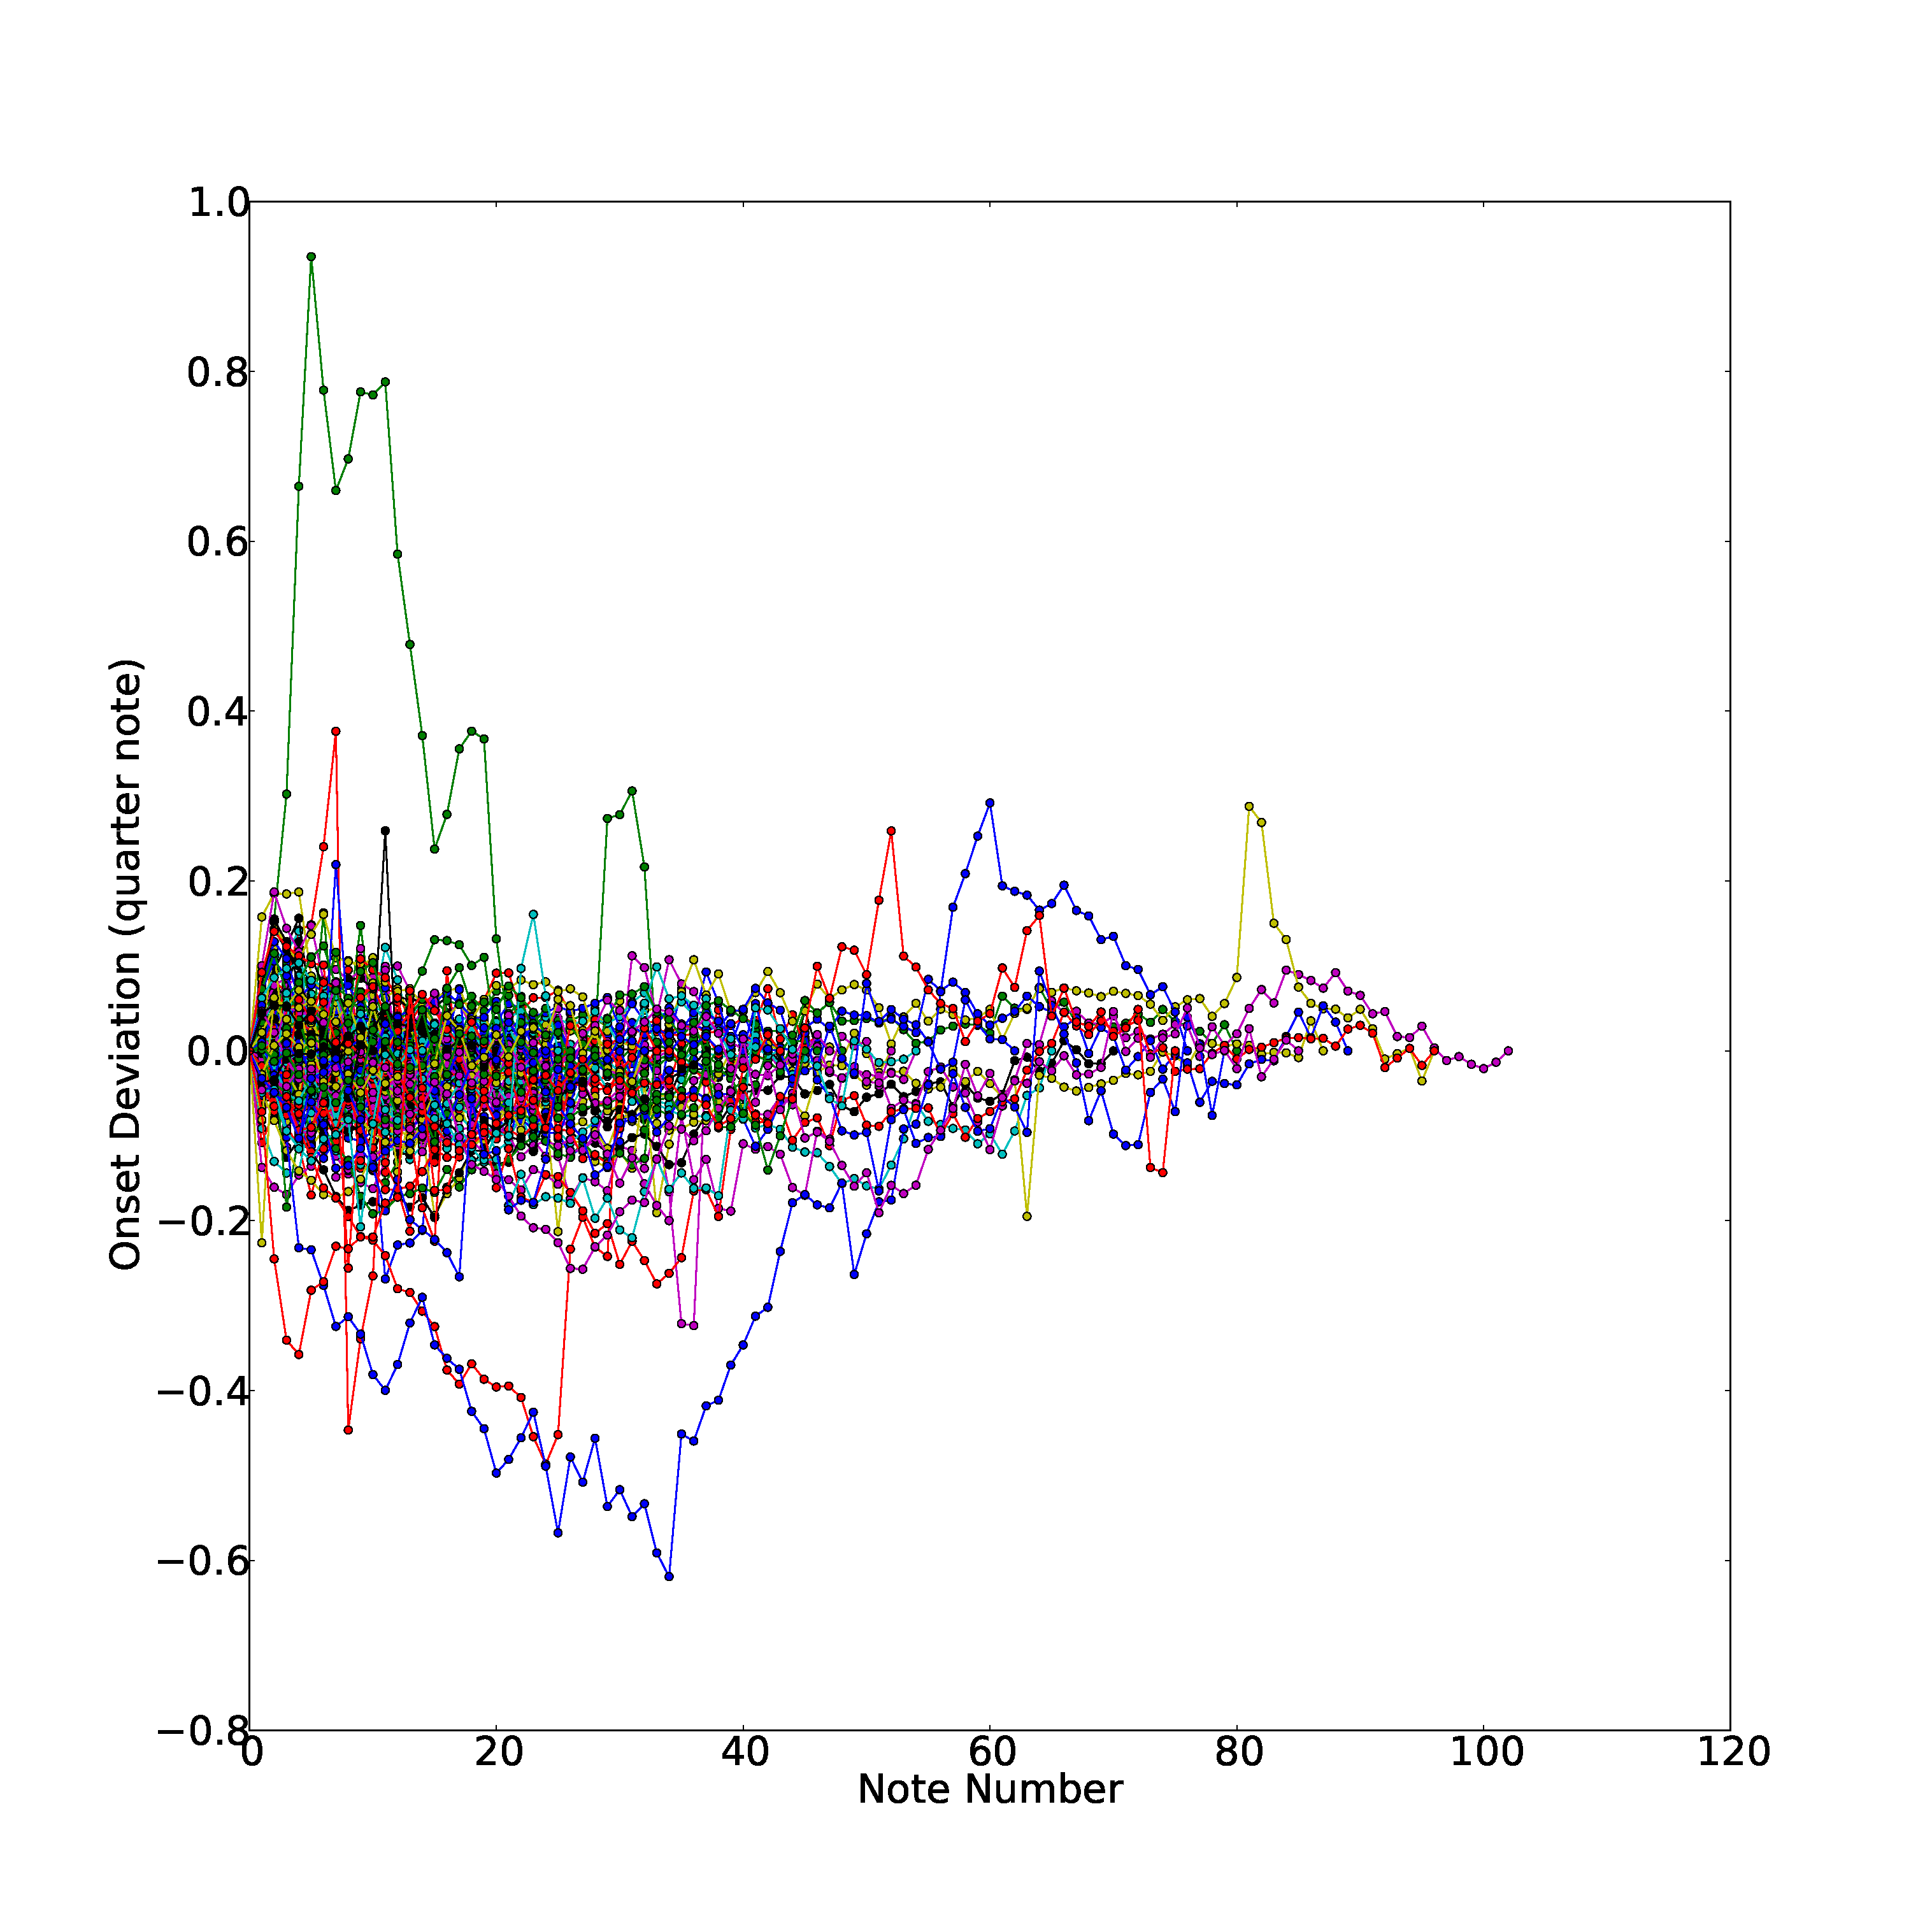
\includegraphics[width=0.8\textwidth]{fig/lian_onset_2}
   \end{center}
   \caption{Onset deviations by aligning last note onset}
   \label{fig:norm1}
\end{figure}

%\begin{figure}[tp]
%   \begin{center}
%      %TODO:Fig.:Normalization Schemes
%      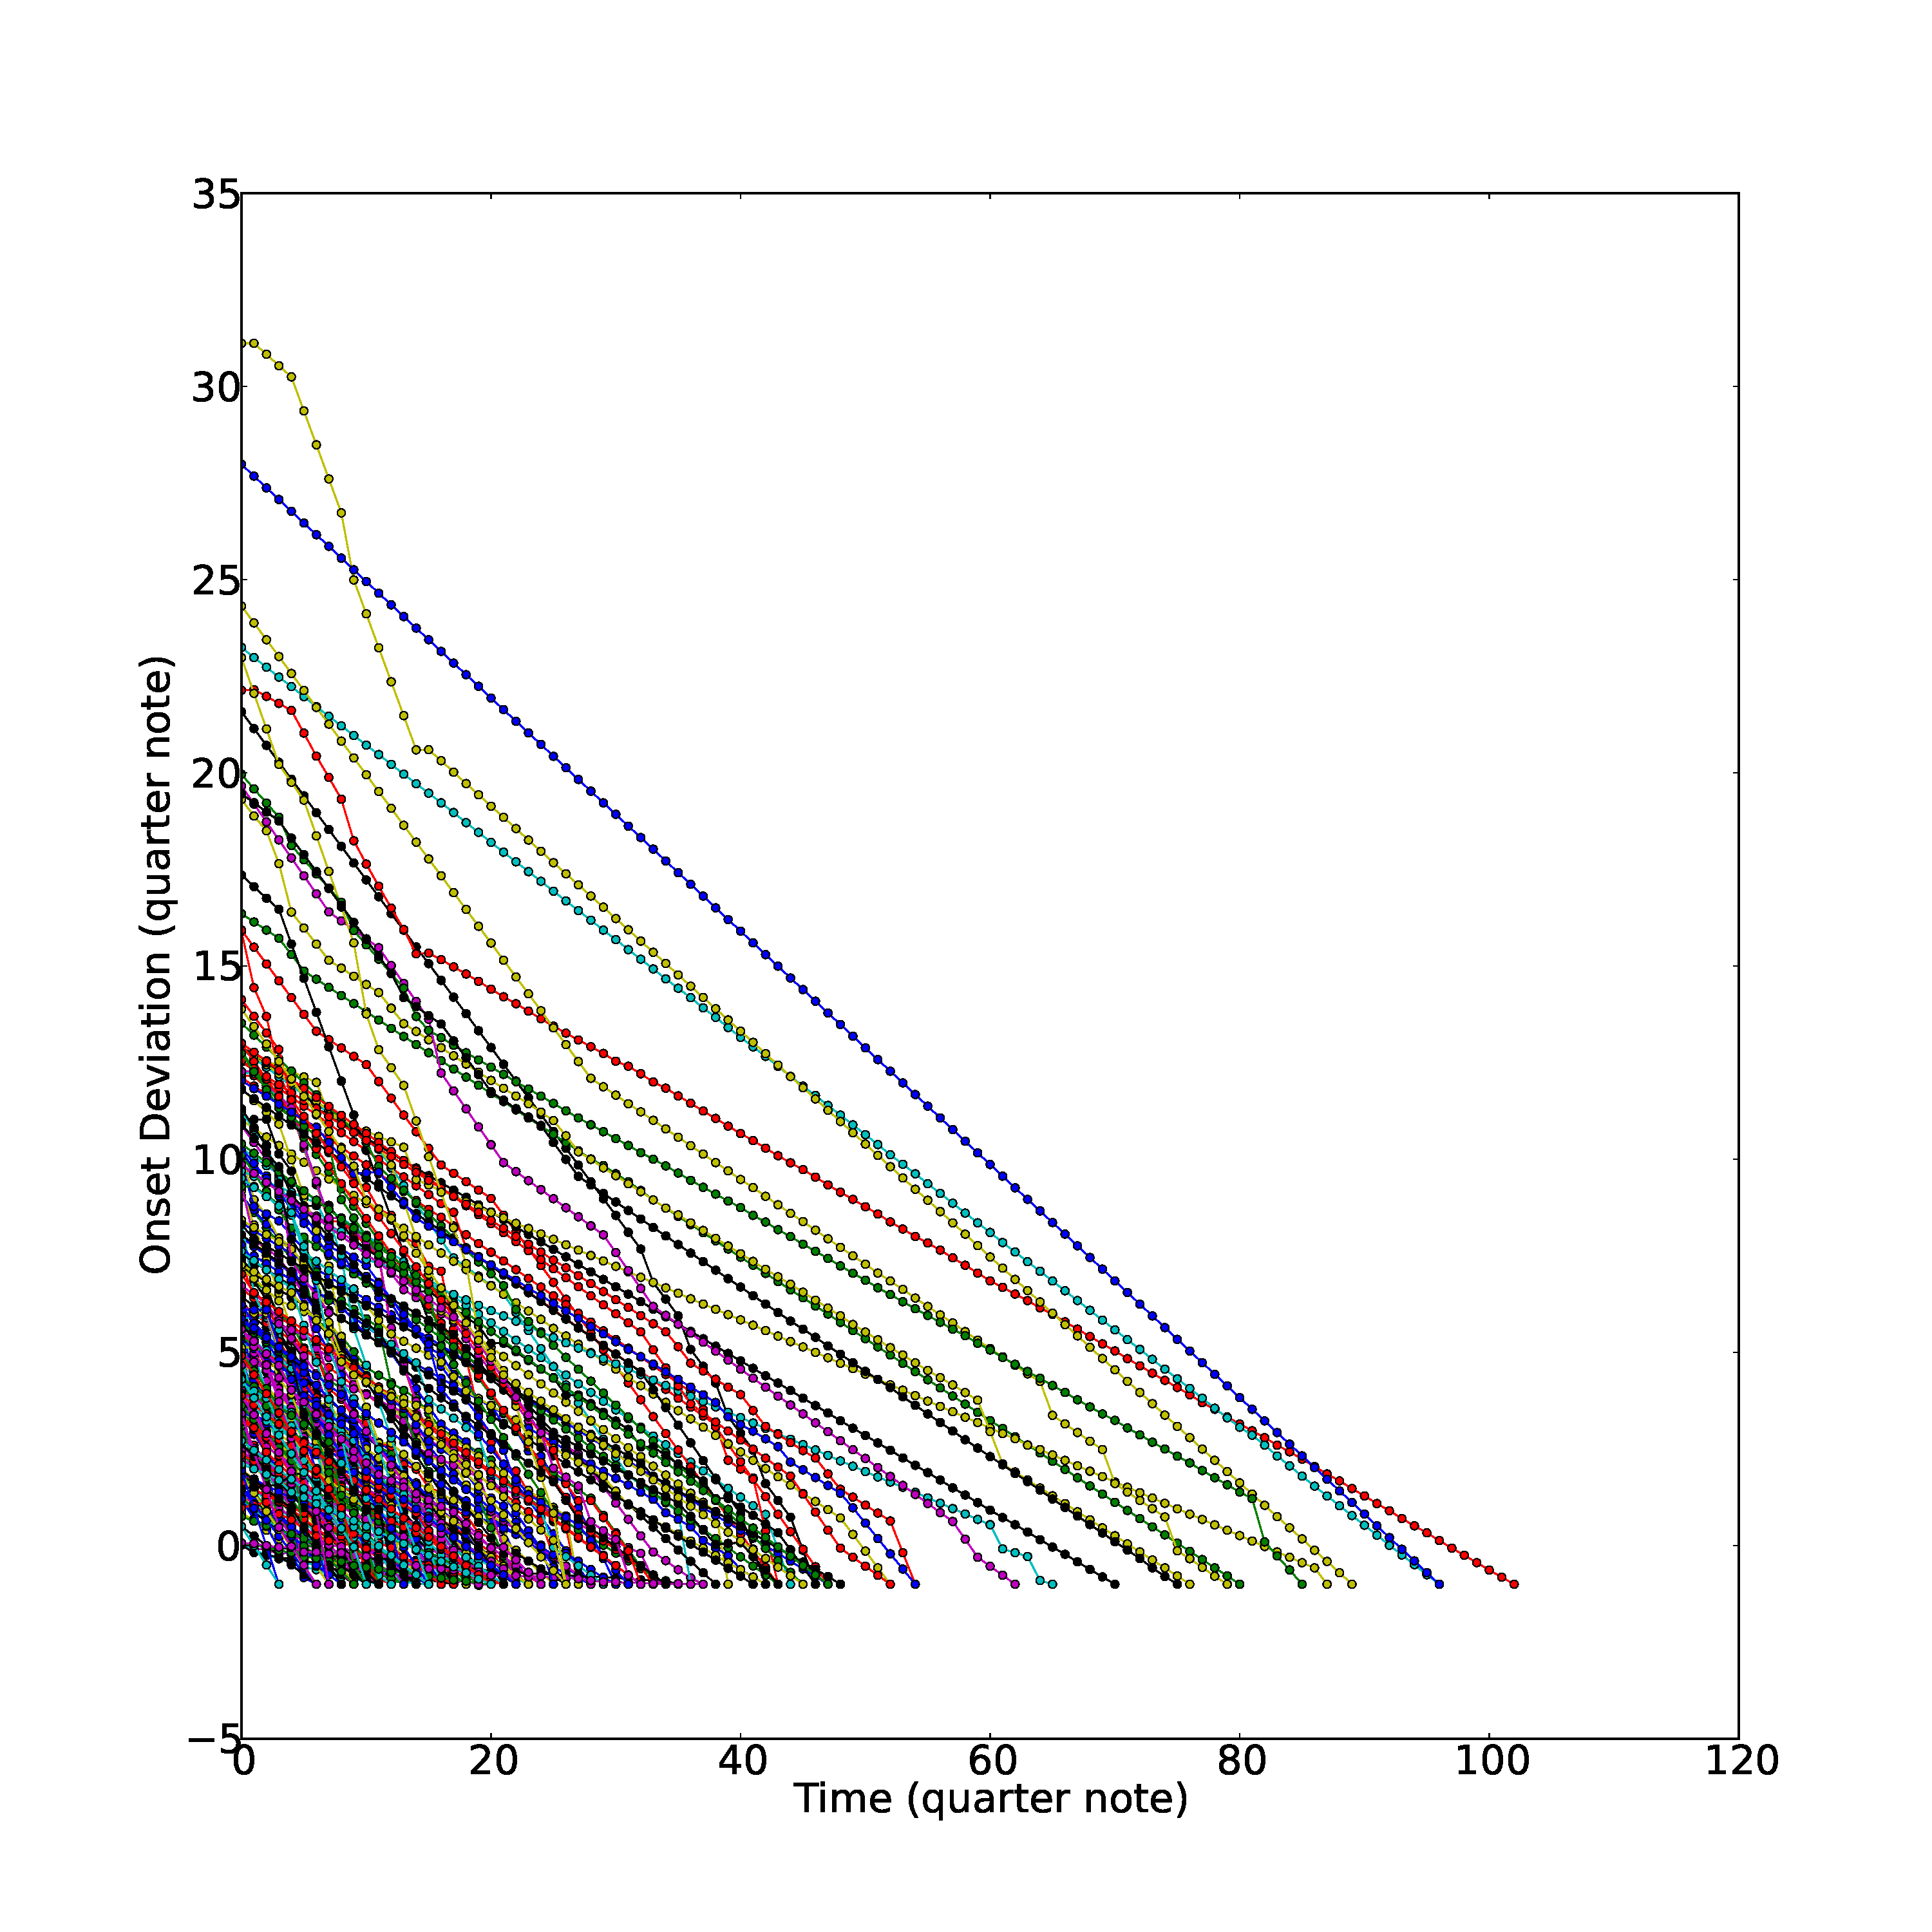
\includegraphics[width=0.6\textwidth]{fig/lian_onset_3}
%   \end{center}
%   \caption{Onset Deviations Using Normalization Method 2}
%   \label{fig:norm2}
%\end{figure}

\begin{figure}[tp]
   \begin{center}
      %TODO:Fig.:Normalization Schemes
      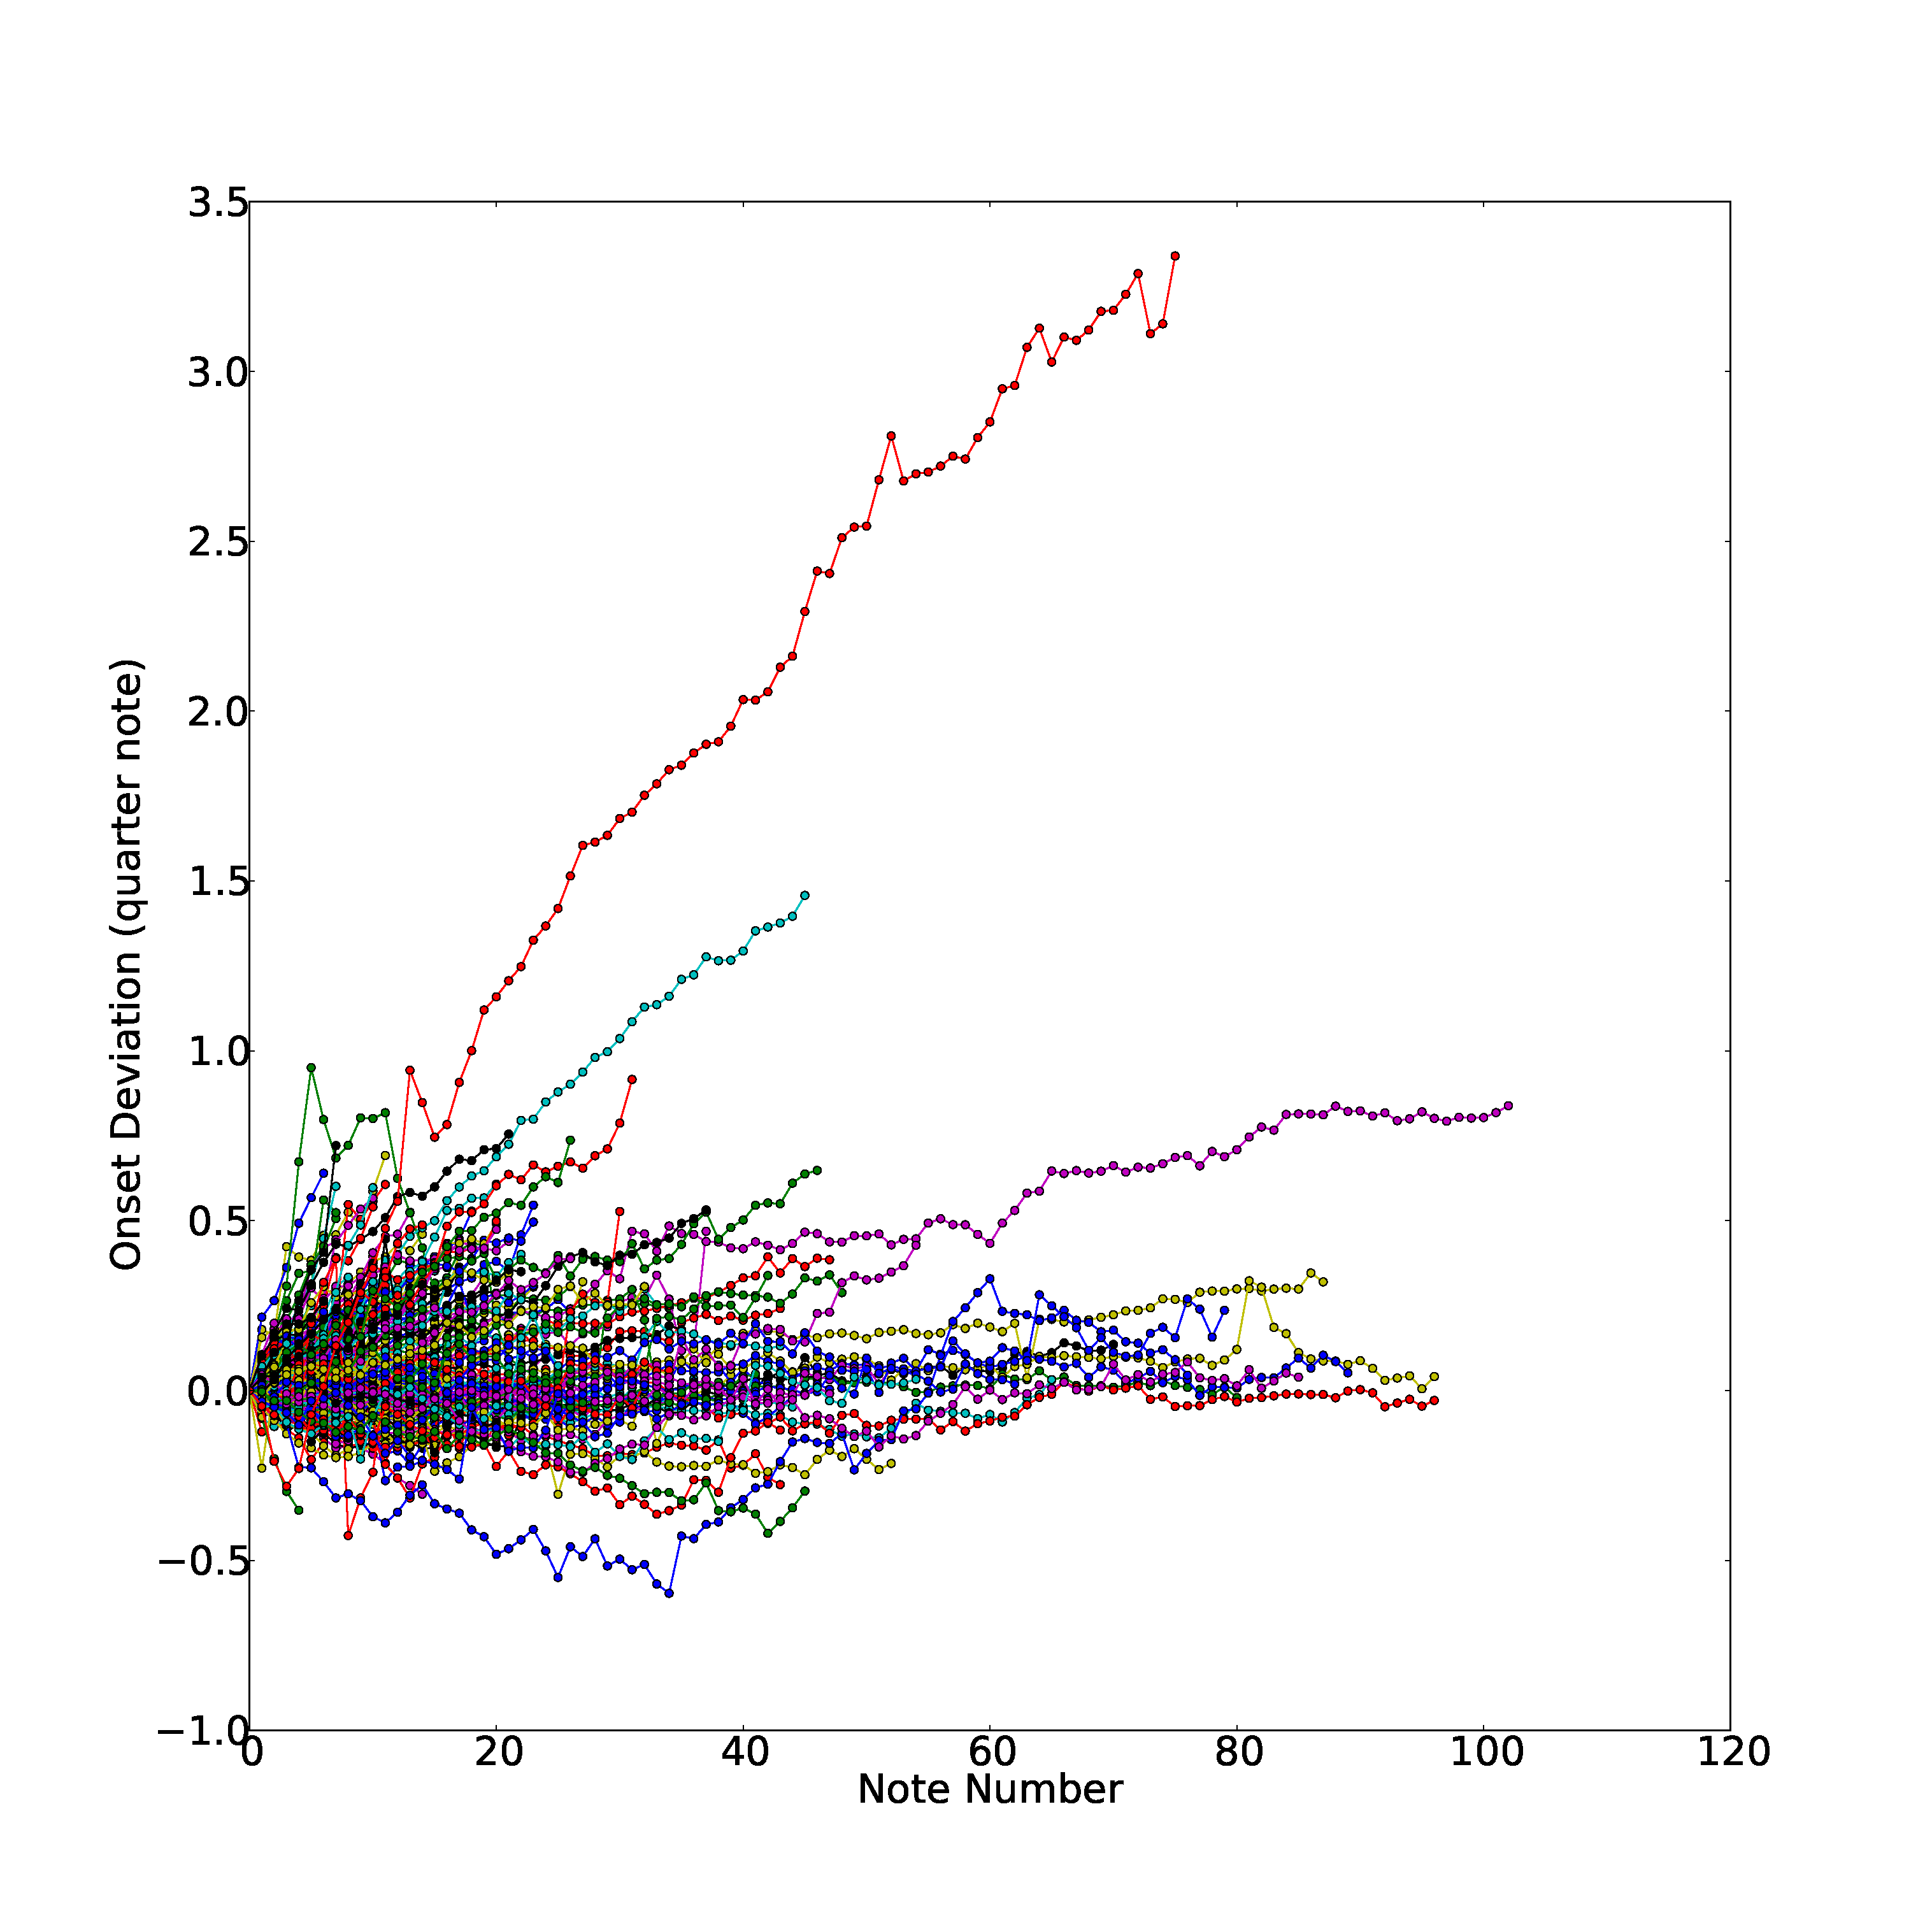
\includegraphics[width=0.8\textwidth]{fig/lian_onset_4}
   \end{center}
   \caption{Onset deviations by aligning last notes note-off}
   \label{fig:norm3}
\end{figure}

%\begin{figure}[tp]
%   \begin{center}
%      %TODO:Fig.:Normalization Schemes
%      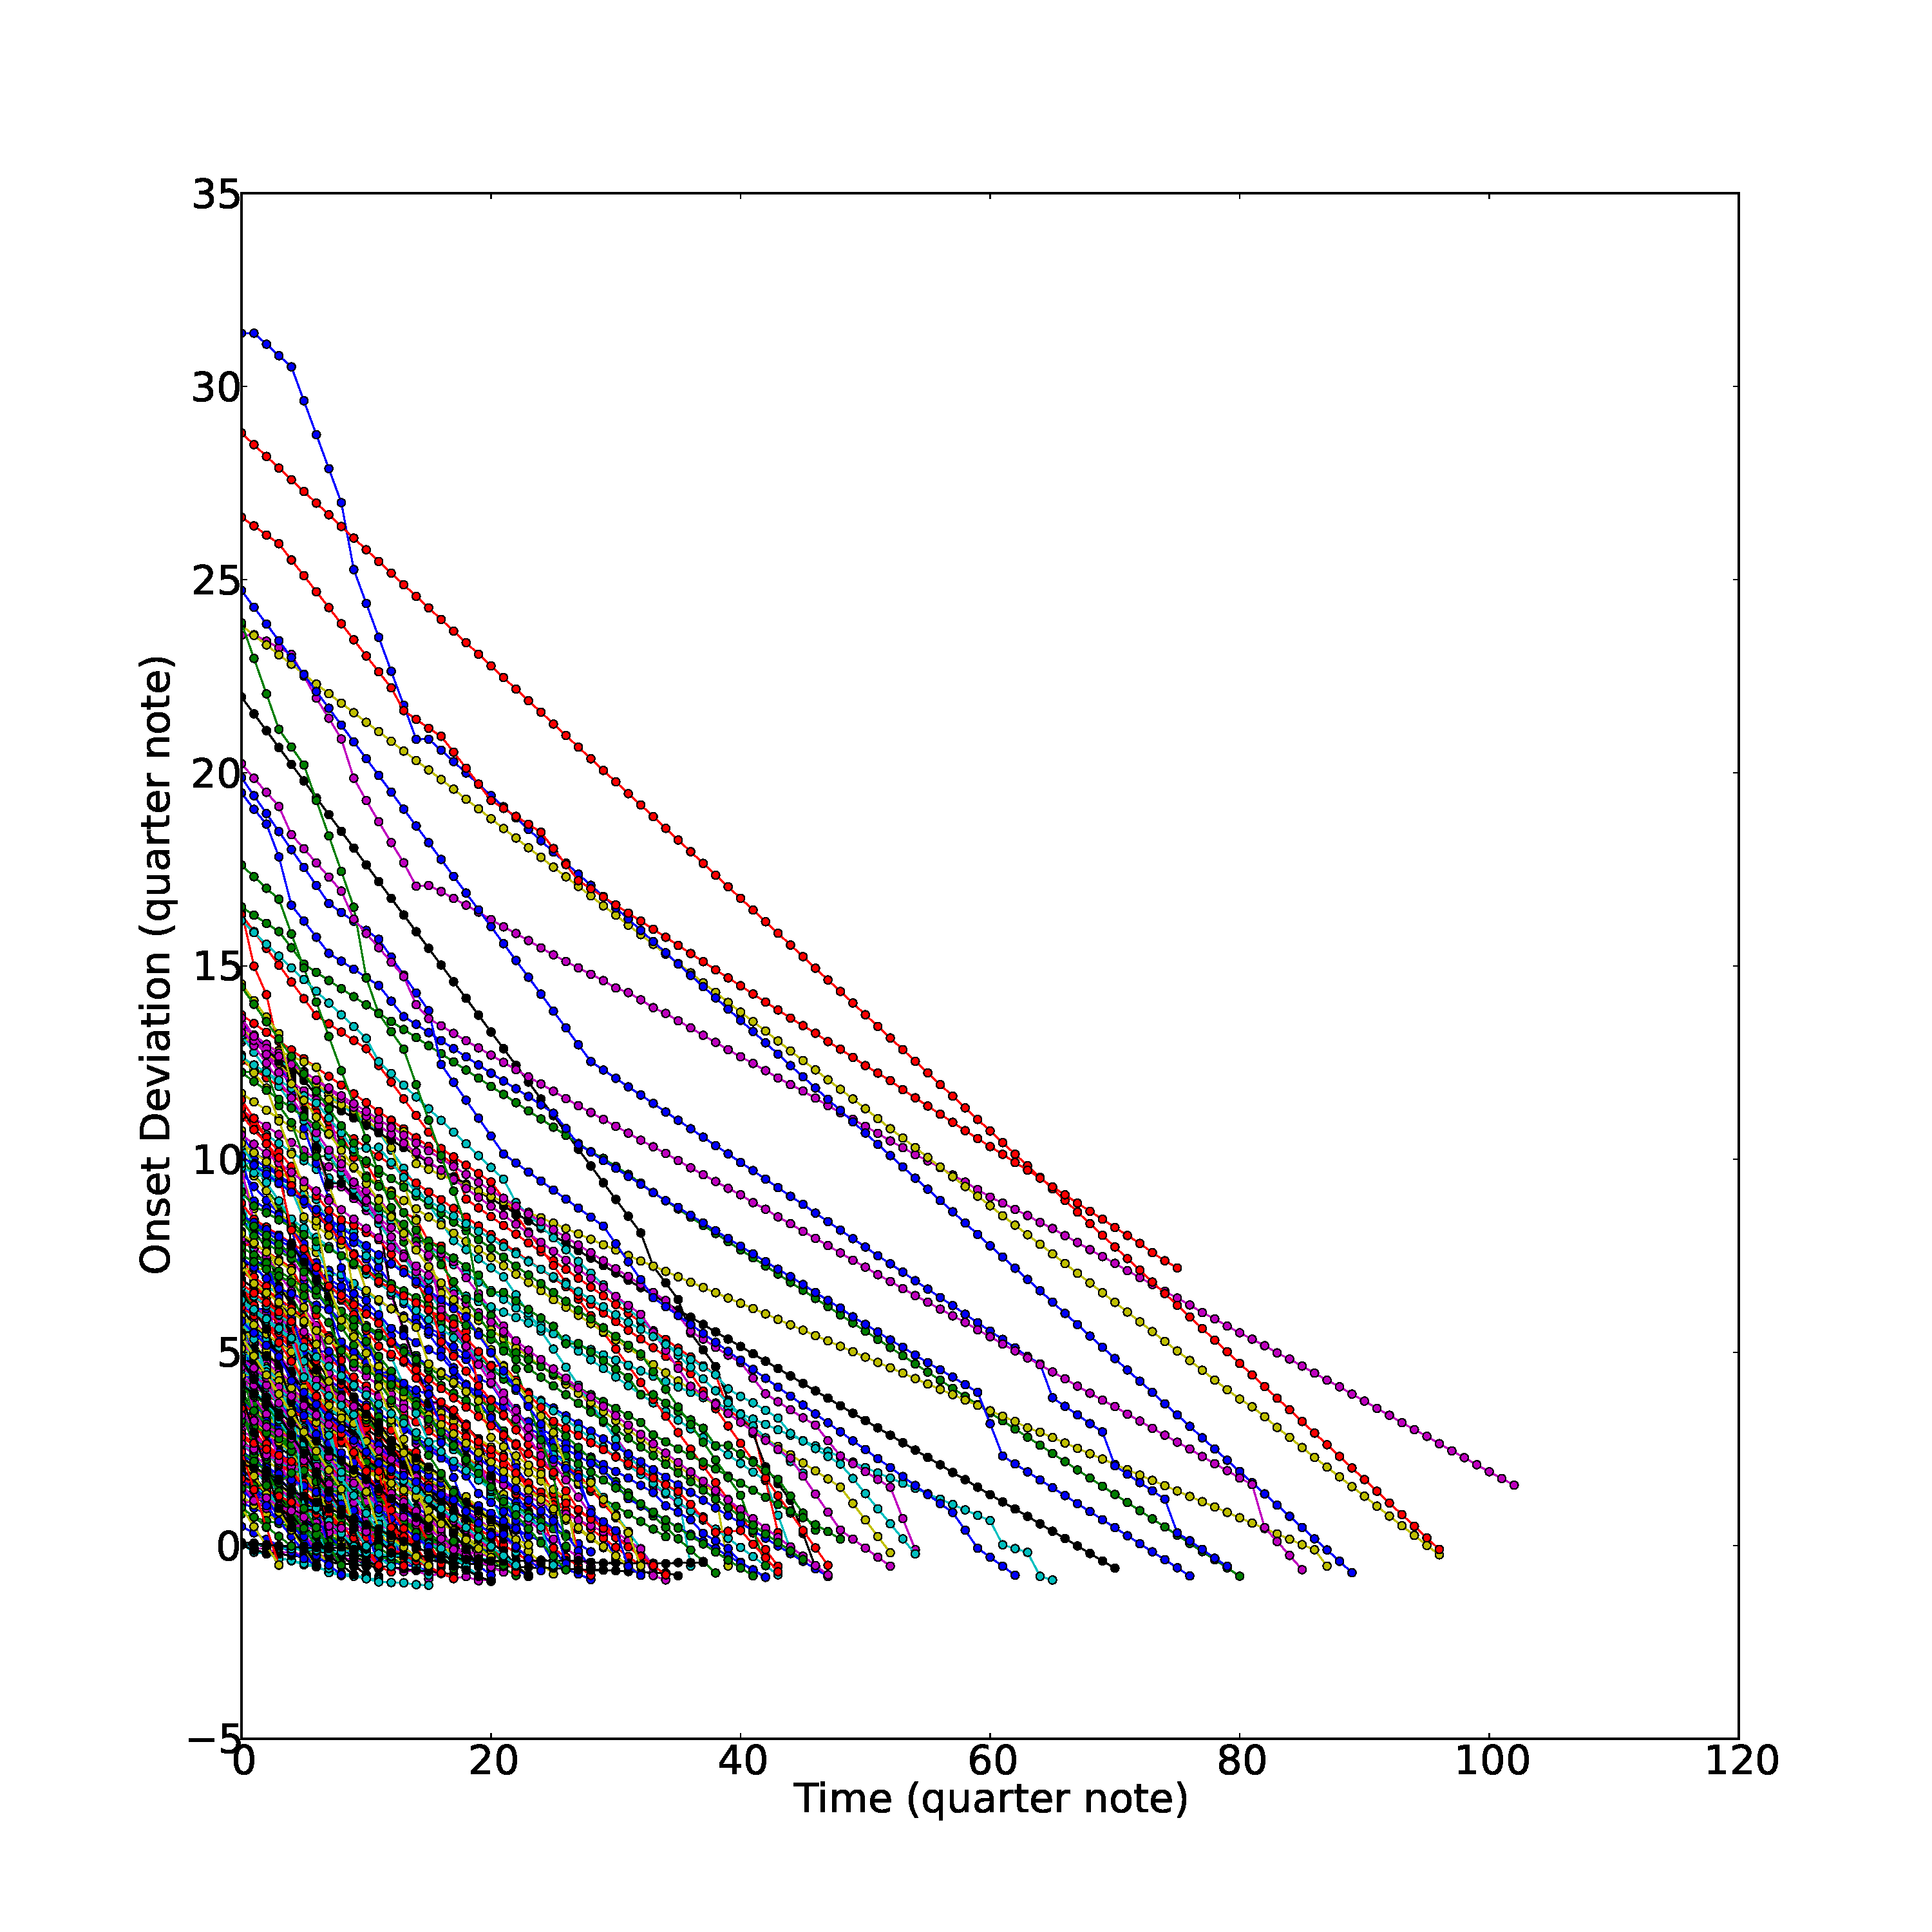
\includegraphics[width=0.6\textwidth]{fig/lian_onset_5}
%   \end{center}
%   \caption{Onset Deviations Using Normalization Method 4}
%   \label{fig:norm4}
%\end{figure}

%\framebox{TODO:remove (quarter note) unit in figures} 
\begin{figure}[tp]
   \begin{center}
      %TODO:Fig.:Normalization Schemes
      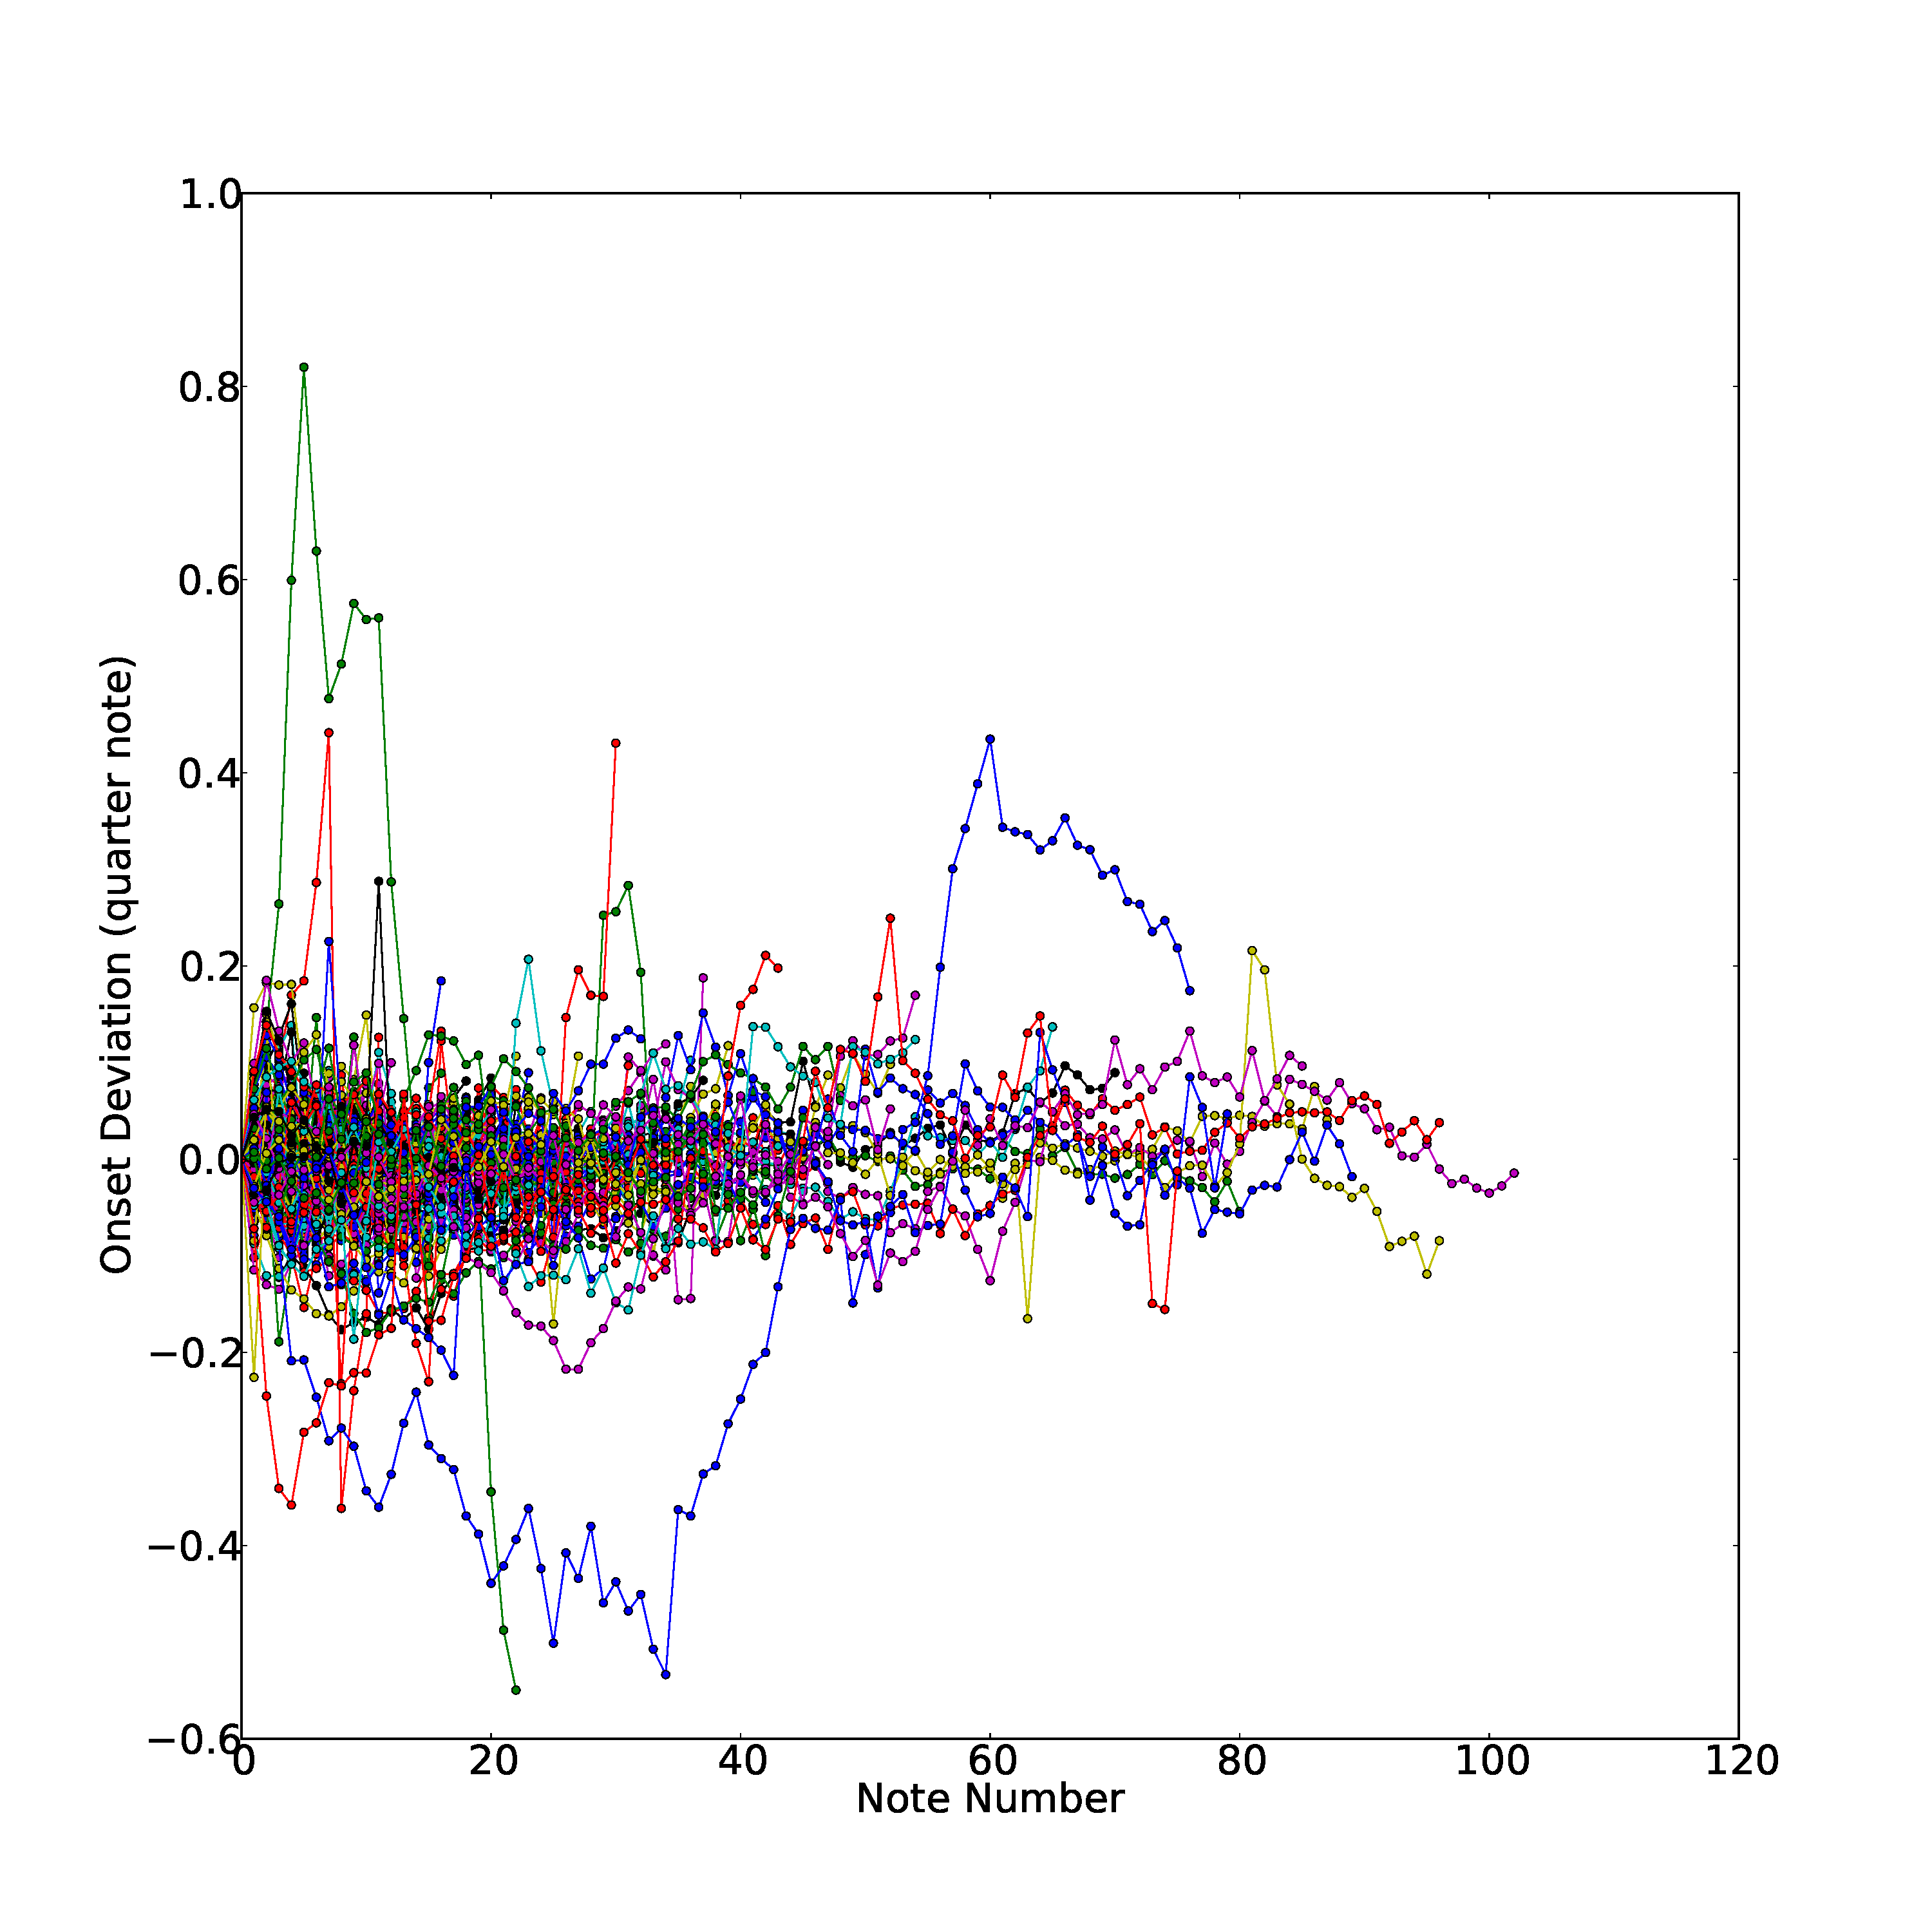
\includegraphics[width=0.8\textwidth]{fig/lian_onset_1}
   \end{center}
   \caption{Onset deviations using automated normalization method}
   \label{fig:normauto}
\end{figure}


\section{Parameter Selection}
\label{sec:paramselect}
\subsection{SVM-HMM-related Parameters}
There are many parameters which need adjustment in SVM-HMM. Two most important parameters, the termination accuracy $\varepsilon$ and the misclassification penalty factor C in SVM, are systematically tested in this experiment to find the optimal value. Since SVM-HMM is an iterative algorithm, the $\varepsilon$ parameter defines the required accuracy for the algorithm to terminate. A smaller $\varepsilon$ will result in higher accuracy, but may take more iterations to compute. The C parameter determines how much weight should be assigned to penalise non-separable samples. A larger C will sacrifice larger margin for lower misclassification error, but it will make the execution time longer.%Therefore, we will leave the rest of the parameters to their default value, and try to find the best C parameter.l

We split performer A's recordings into two sets: the training set includes pieces No.2 to No.6, and the testing set includes piece No.1. We train a model with the training set, and use the learned model to generate the testing set. The generated expressive performance is compared to the corresponding human recordings to calculate the accuracy of the prediction.


%Structural Support Vector Machine has some parameters that needed to be adjusted. We will leave the others to the defaults and change the SVM C trad-off parameter in this experiment. Since three models are learned for three performance features, we have three parameters to adjust. 
%TODO default parameters

%[TODO: phrases count] phrases from [TODO:song counts] songs are used for training. Every first, fifth, and tenth phrases from each song is not included in the training sample, but used as testing samples. A three-by-three grid is layed out for three C parameters, each C takes the value of the powers of tenfrom [TODO: Cs] $10^{-5}$ to $10^4$, so [TODO: num of experiment] paramenters are tested. Then the result is validated
%To measure the effectiveness of the $\varepsilon$ and C parameters, the generated performance is compared to the performance recorded by the performer. 
Ideally, the generated performance will be very similar in expression to the recording. In order to choose the best $\varepsilon$, we calculate the median of similarities between the generated and recorded performances for each $\varepsilon$ choice. Note that each performance feature has its own model, so we will be looking at one performance feature and its $\varepsilon$  parameter at a time. 
First, the generated performance feature sequence and the recorded one are normalized to a range from 0 to 1. This is because the generated performance may have the same up-and-downs as the score, but the value range may be different, so we use normalization to ease our these difference. The Euclidean distance between the two normalized sequences is calculated and divided by the length (number of notes) of the phrase, since the phrase can have arbitrary length. Similar procedure is applied to find the best C.


First we fixed C at $0.1$ and tried different $\varepsilon$'s: $100$, $10$, $1$, $0.75$, $0.5$ and $0.1$. Then, we fix $\varepsilon$ at the optimal value determined in the previous step and test different C's: $10^{-3}$, $10^{-2}$, $10^{-1}$, $0.5$, $1$, and $5$. For each $\varepsilon$ and C combination, we calculate the distance between the generated pieces and recorded examples for all phrases in the testing set for each performer. Then we take the median of all these distances for each $\varepsilon$ or C. The optimal $\varepsilon$ or C is the one that minimize the median of the distances.


%\begin{enumerate}
%	\item Are all the output samples successfully generated? (Generation may fail if the performance features are unreasonable, for example, negative onset timeing.)
%	\item Is the order of the notes preserved? Sometimes the first note is delayed too long and the second note is played too early, so the order is swaped.
%	\item Are there any extreme parameters that makes the expressive performance unnatural?
%\end{enumerate}

%The first two criterias are checked by python scripts, the last one is done by manual inspection.
%
%\framebox{TODO:train / gen corpus}
%\framebox{TODO:how to define distance}
%\framebox{TODO: range of Cs}
%\framebox{TODO: }
%
%\framebox{TODO:experiment result}
%\framebox{TODO: similarity v Cs}
%\framebox{TODO: }
%\framebox{TODO: }
%\framebox{TODO: }
The median distance of the generated performance from the recording for various $\varepsilon$'s are shown in Fig. \ref{fig:eps_accu}. The execution time for various $\varepsilon$'s are shown in Fig. \ref{fig:eps_time}. For $\varepsilon$ value 100 and 10, the termination criteria is too generous so SVM-HMM terminates almost immediately without actually learned anything. Therefore, the outputs are a fixed value for any input. We abandon the data points for $\varepsilon = 100$ or $10$. We can see that the distance drops slowly when $\varepsilon$ becomes smaller. We choose $\varepsilon = 0.1$ for the best accuracy-time tradeoff. %But after $\varepsilon$ is smaller than 0.5, the accuracy doesn't drop anymore. So we will choose $\varepsilon = 0.5 $ for the rest of the experiment to avoid unnecessary computations.

\begin{figure*}[tp]
   \begin{center}
      %TODO:Fig.:Example JSON code
      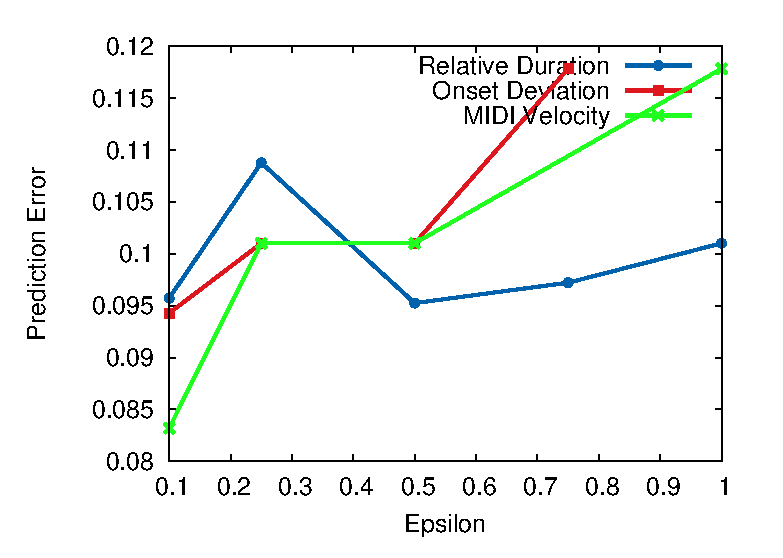
\includegraphics[width=\textwidth]{fig/eps_accu.eps}

   \end{center}
   \caption{Median distance between generated performances and recordings for different $\varepsilon$'s}
   \label{fig:eps_accu}
\end{figure*}
\begin{figure*}[tp]
   \begin{center}
      %TODO:Fig.:Example JSON code
      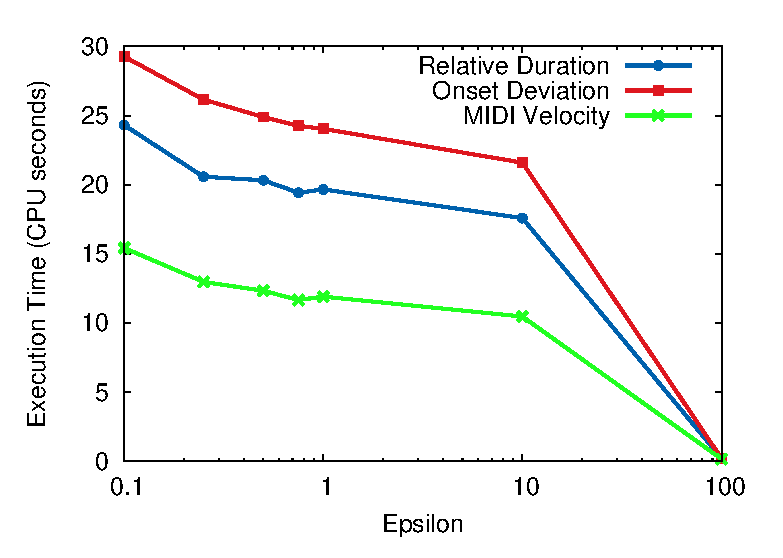
\includegraphics[width=\textwidth]{fig/eps_time.eps}

   \end{center}
   \caption{Execution time for different $\varepsilon$'s}
   \label{fig:eps_time}
\end{figure*}

As for different C parameter, the accuracy and execution time are shown in Fig. \ref{fig:c_accu} and Fig. \ref{fig:c_time}, respectively. We can't find a clear trend in Fig. \ref{fig:c_accu}, but we can find that for C over $10$ and under $0.01$, the model failed to produce meaning fule model (i.e. the output is a fixed value), so the data point is omitted in the figure. Therefore, choosing a C in the middle will produce more robust model. In Fig. \ref{fig:c_time} the execution time grows as C goes larger, so considereing the robustness (always producing meaningful model) and time tradeoff, we choose C = 0.1 as our optimal C.

\begin{figure*}[tp]
   \begin{center}
      %TODO:Fig.:Example JSON code
      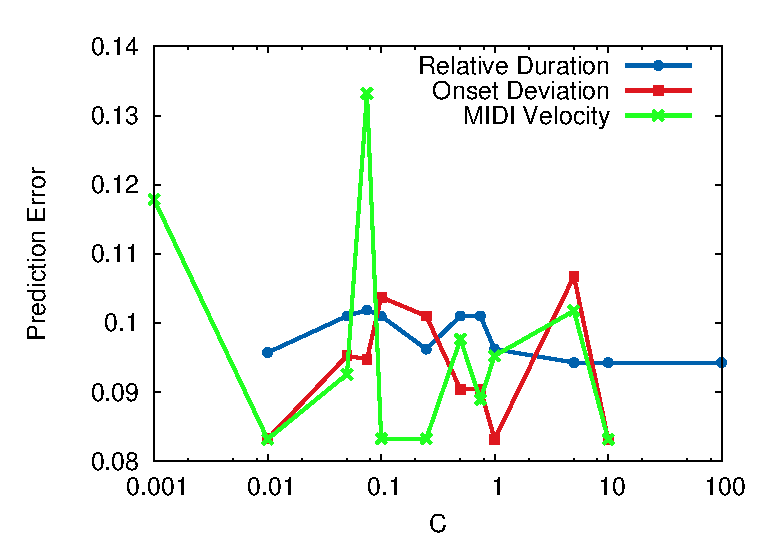
\includegraphics[width=\textwidth]{fig/C_accu}

   \end{center}
   \caption{Median distance between generated performances and recordings for different C's}
   \label{fig:c_accu}
\end{figure*}
\begin{figure*}[tp]
   \begin{center}
      %TODO:Fig.:Example JSON code
      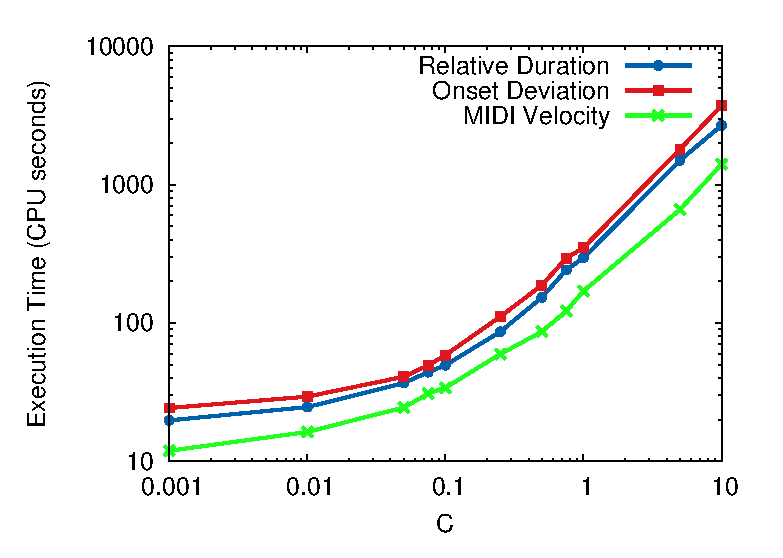
\includegraphics[width=\textwidth]{fig/C_time}
   \end{center}
   \caption{Execution time for different C's}
   \label{fig:c_time}
\end{figure*}
\subsection{Quantization Parameter}
Besides $\varepsilon$ and C, the number of quantization levels for SVM-HMM input is also has some impact on the execution time. If the performance features are quantized into more fine-grained levels, the quantization errors can be reduced, but the execution time and memory usage will grow dramatically. Also, larger number of intervals doesn't imply more accurate or robust model. Because SVM-HMM is originally used in part-of-speech tagging problem, if we use divide the performance features into more intervals, there will be fewer samples in each interval. But from a statistical learning point of view, it is desirable to have fewer bins with more samples in each, rather than a large number of bins with very sparse samples in each. To illustrate this point, consider a three note segment is played once in the following MIDI velocity: (60, 70, 80), and the same segment is played again in (60.1, 69.9, 80.1). If we have a quantization interval width of, say, 0.05, then 60 and 60.1 may be quantized into different bins, and 70 and 69.9 may also be quantized into different bins, so the two phrases will be considered as two different case. However, if the quantization interval width is 1, both phrases may be quantized into the same label sequence, which is more desirable because the SVM-HMM algorithm can capture the similarity in the two samples. 

Initially, we tried to quantized the values into 1025 uniform width bins, wishing to minimize the quantization error. But it take very long (hours, even days) to learn a model, and the output only falls on a very sparse set of values. So we reduce this number to 128. This level of quantization is fine enough to capture the performance nuance. Taking a rough estimate, onset deviation feature rarely exceeds $\pm 1$, so the quantization interval width is around $\frac{1-(-1)}{128} = 0.015625$. Most duration ratios falls between zero and three, so the interval width is $\frac{3-0}{128} = 0.0234375$. MIDI velocity is roughly around 30 to 90, so the interval is about $\frac{90-30}{128} = 0.46875$. This level of granularity is good enough for our performance system, and can dramatically reduce the execution time without sacrificing the expressiveness of the models. 

We repeated the $\varepsilon$ selection experiment for quantization level of 1025 and 128. The execution time (in CPU second) is shown in Fig. \ref{fig:quant_comp}. The time required for 1025 is larger than 128 by orders of magnitudes, but the expressiveness does not improve much.%The expressiveness of the output is even improved (evaluated by subjective listening).

\begin{figure}[tp]
   \begin{center}
      %TODO:Fig.:Normalization Schemes
      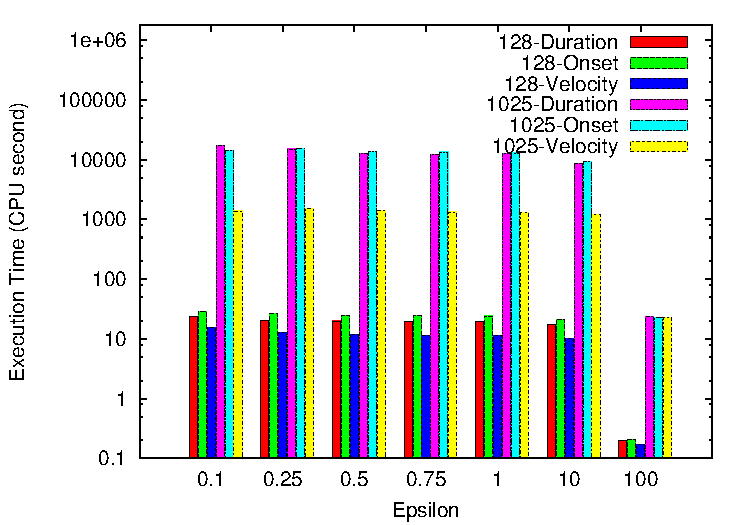
\includegraphics[width=\textwidth]{fig/quant_comp}
   \end{center}
   \caption{Execution time for differnt number of quantization levels}
   \label{fig:quant_comp}
\end{figure}

\section{Human-like Performance}
\label{sec:turing}
The goal of our system is to create expressive, non-robotic music as oppose to deadpan MIDI. Therefore, we need to perform a subjective test to verify if people can tell our generated performances apart from real human performances.

In this survey, 1518 computer generated expressive phrases and their corresponding human recording were selected as samples. Each test subject was given 10 randomly selected computer generated phrase and 10 human recordings, these 20 phrases are presented in random order. He/She was asked to rate each phrase according to the following criteria, which were proposed by the RenCon contess \cite{RenCon}:
\begin{enumerate}
   \item Technical control: if a performance sounds like it is technically skilled thus performed with accurate and secure notes, rhythms, tempo and articulation.
   \item  Humanness: if the performance sounds like a human was playing it.
   \item  Musicality: how musical the performance is in terms of tone and color, phrasing, flow, mood and emotions
   \item Expressive variation: how much expressive variation (versus deadpan) there is in the performance.
\end{enumerate}

In RenCon, each judge was asked to give separate ratings for each criteria. But we believe this is too demanding for less-experienced participant, so we asked each test subject to give an overall rating from one to five. One being very bad, five being very good. The test subjects are also asked to report their musical proficiency in a three level scale:
\begin{enumerate}
   \item No experience in music 
   \item Amateur performer
   \item Professional musician, musicologist or student majored in music
\end{enumerate}

To generate the expressive performance phrase. We follow a six-fold cross-validation pattern: for each performer in the corpus, we use all his/her recorded phrases of Clementi's Op.36 No.2 to No.6 to train a model. Then the model is used to generate all phrases from Clementi's Op.36 No.1. The generate phrases and the performer's recordings of piece No.1 will all be included as samples. The process is repeated, but each time the piece excluded for training will be changed to No.2, No.3 and so on. So all six pieces will have a computer generated version (trained by each player's corpus) and a recorded version.

%With these music material ready, we built a survey web page to let the test subjects vote. A test subject was first asked to report their music proficiency (No music training at all, amateur or professional musician/scholar/student) and musical instrument skill. Then he/she will be asked to identify the computer generated phrase from a generated/recorded pair. Five pairs will be randomly selected from all the available pairs, and the order of appearance of the generated and recorded one will be randomized.

We have also tried using all performers' recordings to train a single model. However, the expressive variation from that model is much smaller than a model trained by a single performer's recordings. This is because expression from different performers may cancel each other out. This phenomena can be found in the distribution histograms for each performance features (Fig. \ref{fig:distonset}, Fig. \ref{fig:distdur} and Fig. \ref{fig:distvel}). The features generated from the full corpus are slightly more concentrated, which results in less dramatic expression.


\begin{figure}[tp]
   \begin{center}
      %TODO:Fig.:Normalization Schemes
      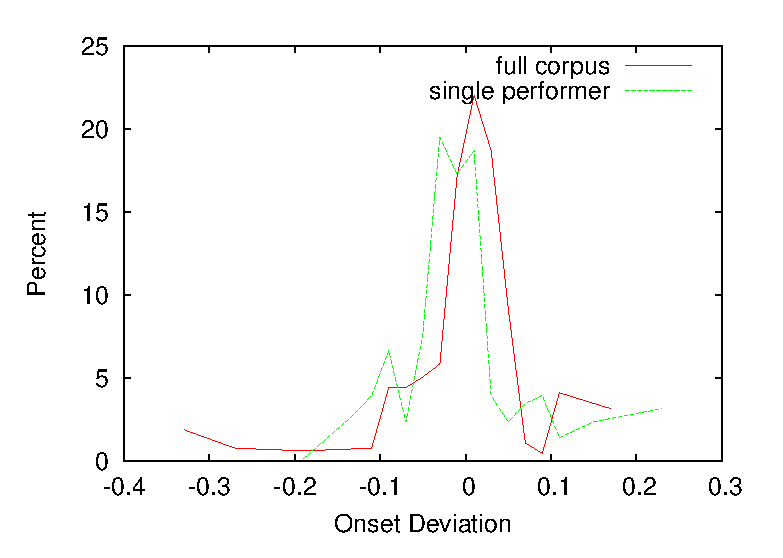
\includegraphics[width=0.8\textwidth]{fig/all_01_onset}
   \end{center}
   \caption{Distribution of onset deviation values from full corpus versus single performer's corpus}
   \label{fig:distonset}
\end{figure}
\begin{figure}[tp]
   \begin{center}
      %TODO:Fig.:Normalization Schemes
      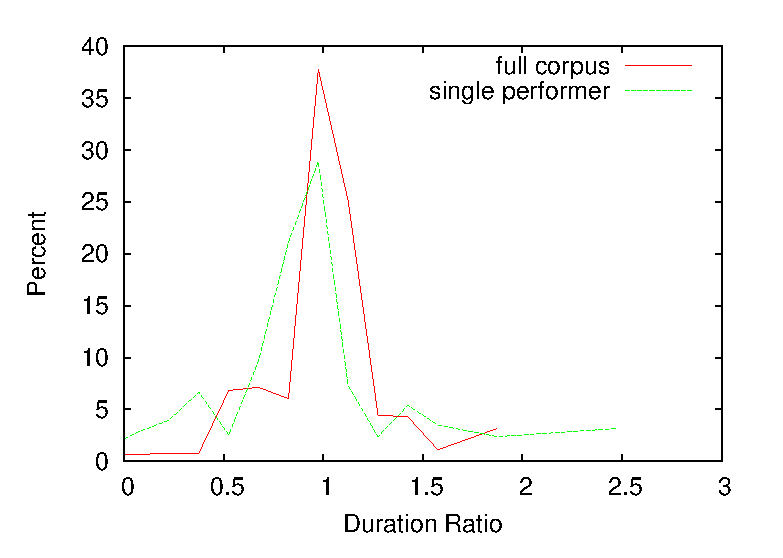
\includegraphics[width=0.8\textwidth]{fig/all_01_duration}
   \end{center}
   \caption{Distribution of duration ratio values from full corpus versus single performer's Corpus}
   \label{fig:distdur}
\end{figure}
\begin{figure}[tp]
   \begin{center}
      %TODO:Fig.:Normalization Schemes
      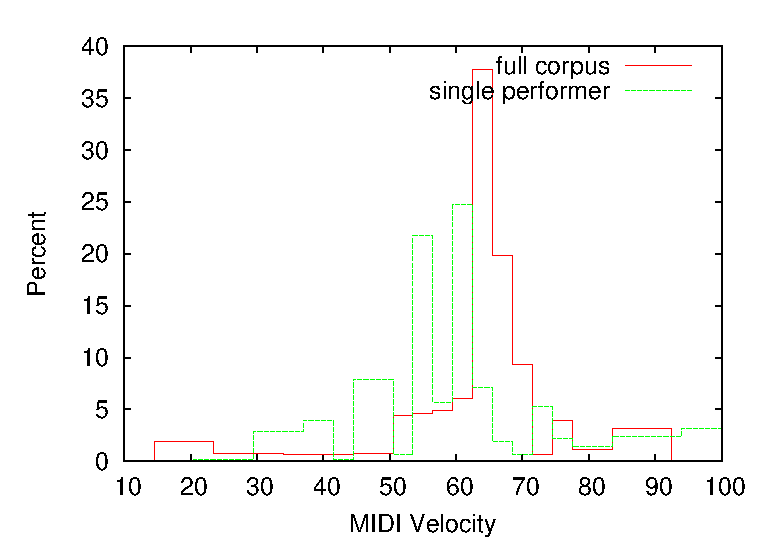
\includegraphics[width=0.8\textwidth]{fig/all_01_velocity}
   \end{center}
   \caption{Distribution of MIDI velocity values from full corpus versus single performer's corpus}
   \label{fig:distvel}
\end{figure}


%\framebox{TODO:Turing test result and discussion}

%We distributed a web survey to check if our computer generated performance are indistinguishable to human recordings. The expressive performance generated by the method described above are collected, as well as all human recordings from the corpus. Each participant will be given ten random phrases from the computer generated phrases, and ten random phrases from human recordings. The twenty phrases will be presented in random order. The participant are asked to give 

We received 119 valid samples for the survey. Fifty of them are from people with no music background, 59 are from amateur musicians, and the rest 10 are from professional musicians. The average rating given to computer generated performances and human recordings are listed in Table \ref{tab:avg_rating}. It is clear that for professional and amateur musician, the average rating given to human performances are higher than computer performances. However, for participants who have no experience in music, the ratings are much closer. A Student T-test on the two ratings given by participants with no experience yields a p-value of 0.0312, therefore we can't reject the null hypothesis that the two ratings are different under a significance level of 99\%. Therefore we can say for participants with no music experience, the computer generated music and human recordings are indistinguishable.


\begin{table}
   \centering
   \caption{Average rating for generated performance and human recording}
   \label{tab:avg_rating}
   \begin{tabular}{r|rr}
      \hline
      &Computer &Human \\
      \hline
      No experience&3.243&3.391\\
      Amateur&2.798&3.289\\
      Professional&2.430&3.010\\
      \hline
      Total&2.952&3.306\\
      \hline
   \end{tabular}
\end{table}

In order to get more insight from the ratings, we can further divide the performers in the corpus into two categories by their piano skill level. By the number of mistakes made (Table \ref{tab:mistakes}), performer A and B are considered more skillful than performer C, D, E and F. The average ratings given to the performances generated from the model trained by samples of the two categories are listed in Table \ref{tab:good-bad_rating}. The distance between computer and human performances are smaller for less-skillful group (C to F) than the skillful group (A and B). This is probably because our system makes some mistakes that are similar to the mistakes made by less-skillful performers. For example, unsteady tempo, sudden change in loudness, hesitation are all common problems that exists in both less-skillful performance and computer generated performance. But for skillful performers, who have better technical control and have better sense of musical structure, the problems described above will happen less often. This will make the generated works sound much worse comparing to the better performance.%This is probably because our system still can't capture every nuance of human performances.

\begin{table}
   \centering
   \caption{Average rating for generated performance and human recording under different part of the corpus}
   \label{tab:good-bad_rating}
   \begin{tabular}{r|rr|rr}
\hline
&A,B&&C-F&\\
&Computer &Human &Computer &Human \\
\hline
No experience&3.067&3.302&3.363&3.451\\
Amateur&2.680&3.347&2.863&3.286\\
Professional&2.048&3.162&2.708&2.921\\
\hline
Total&2.776&3.313&3.066&3.323\\
\hline
   \end{tabular}
\end{table}

If we look into each individual participant, we can check if a participant gives higher (average) rating to computer or human performances, or equal ratings for both. The number of participants who fall into each categories are shown in Table \ref{tab:avg_count}. Twenty-six of the non-experienced participants give higher or equal rating to computer than human, slightly higher than twenty-four people who gives higher rating to human. For amateur and professional musicians, the number of people who prefers human are much higher. In Table \ref{tab:good-bad_count}  the generated performances are split into  two categories just like Table \ref{tab:good-bad_rating}. The results are similar to Table \ref{tab:avg_count}: the difference between computer and human is higher for skillful performers (A and B) than less-skillful performers (C to F).
Therefore we can conclude that our system has the same expressive power for participants with no music background. But for amateur and professional musician, the system requires further improvements to be comparable to human musician.

\begin{table}
   \centering
   \caption{Number of participants who gives higher rating to generated performance, human recordings or equal rating}
   \label{tab:avg_count}
   \begin{tabular}{r|rrr|r}
      \hline
      &Computer&Equal&Human&Total\\
      \hline
      No experience&19&7&24&50\\
      Amateur&7&3&49&59\\
      Professional&1&1&8&10\\
      \hline
      Total&27&11&81&119\\
      \hline
   \end{tabular}
\end{table}

\begin{table}
   \centering
   \caption{Number of participants who gives higher rating to generated performance, human recordings or equal rating under different part of the corpus}
   \label{tab:good-bad_count}
   \begin{tabular}{r|rrr|rrr|r}
\hline
&&A,B&&&C-F&&Total\\
&Computer&Equal&Human&Computer&Equal&Human&\\
      \hline
No experience&5&4&6&14&3&18&50\\
Amateur&2&1&18&5&2&31&59\\
Professional&0&1&3&1&0&5&10\\
      \hline
Total Result&7&6&27&20&5&54&119\\
      \hline
   \end{tabular}
\end{table}


